\chapter{Background and Theory}
% This chapter should describe the theoretical background needed to understand
% and solve the problem. For instance, a description of the hardware platform
% or specific components involved in this assignment, definition of concepts
% that are important to understand the solution should be summarized here. Add
% citations to show sources whenever appropriate.

This chapter contains background theory relevant to the exercise. The first part is a brief introduction to the various hardware components of the EFM32GG-DK3750 that were used in this exercise. The second part details energy optimization techniques in modern computing systems. Finally, a small section outlines theory of soundwaves and music.


\section{Overview of EFM32GG-DK3750}
Through the exercises in this course we are working with the Silicon labs EFM32GG-DK3750 prototyping board (figure \ref{fig:efm-board}), from here on referenced as EFM32GG. The EFM32GG hardware components we used in this exercise include the following:
\begin{itemize}
	\item Clock Management Unit
	\item Timer/Counter
	\item Digital to Analog Converter
	\item General-Purpose Input/Output pins
	\item Gamepad Prototype
	\item Energy Management Unit
  \item Low Energy Timer
  \item Peripheral Reflex System
%  \item Low Energy Universal Asynchronous Receiver/Transmitter
	\item Direct Memory Access controller
  % TODO: Add the components used in exercise 2 to this list
\end{itemize}
A more comprehensive map of the EFM32GG hardware components is shown in figure \ref{fig:giant-gecko-map}.

\begin{figure}[H]
  \centering
  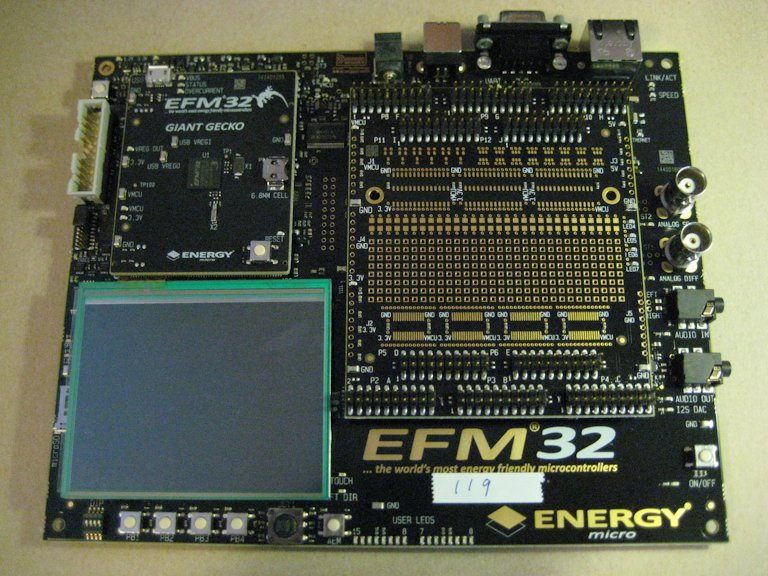
\includegraphics[width=0.7\textwidth]{images/efm_board.jpg}
  \caption{The EFM32GG prototyping board}\label{fig:efm-board}
\end{figure}

\begin{figure}[H]
  \centering
  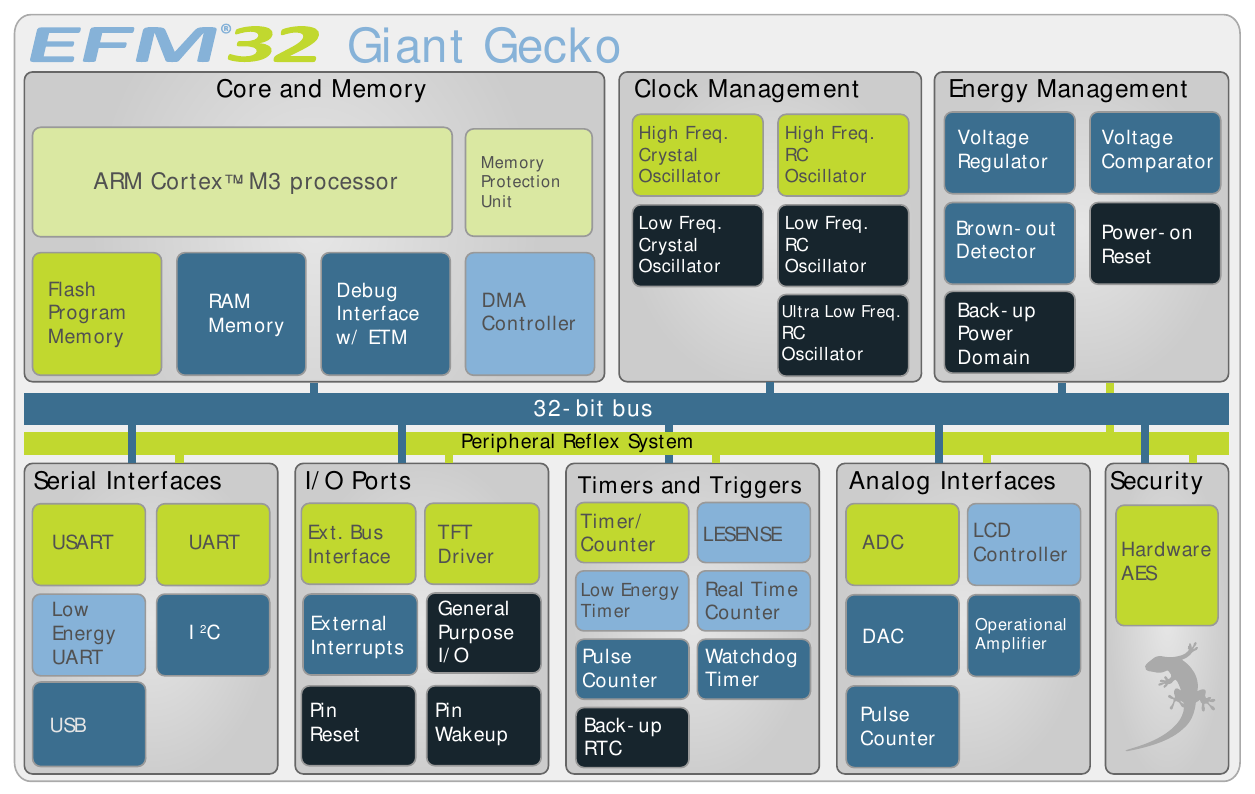
\includegraphics[width=\textwidth]{images/giant_gecko_map.png}
  \caption{Map of the EFM32GG hardware components}\label{fig:giant-gecko-map}
\end{figure}


\section{Clock Management Unit}\label{sec:cmu}
The Clock Management Unit (CMU) controls the on-board oscillators and clocks, and produces clock signals that drives the core modules and all the peripherals. The CMU can be used to enable or disable clock signals for the different peripherals on an individual basis. It possible to reduce the power consumption significantly by only enabling the clock for the peripherals that will be used. By default, the clock signals for all peripherals is disabled. 

The CMU manages several system clocks in order to provide different clock signals to core modules and peripherals. These clocks include the High Frequency Clock (HFCLK), the High Frequency Core Clock (HFCORECLK), and the High Frequency Peripheral Clock (HFPERCLK).\cite{efm32gg-rm}

\subsection{High Frequency Clock}
HFCLK drives two prescalers that generate HFCORECLK and HFPERCLK, in addition to driving the CMU itself. With separate prescalers it is possible to configure the clock speeds of the core modules and the peripherals individually. The HFCLK itself can be driven either by one of the high-frequency oscillators (HFRCO and HFXO), or by one of the low-frequency oscillators (LFRCO and LFXO). 

\subsection{High Frequency Core Clock}
HFCORECLK is the clock that drives the core modules, which consists of the CPU and tightly coupled modules such as the DMA. The frequency of HFCORECLK can be changed dynamically by writing to CMU\_HFCORECLKDIV, and the clock can be disabled for individual modules by clearing bits in CMU\_HFCORECLKEN0. 

\subsection{High Frequency Peripheral Clock}
HFPERCLK is the clock that drives the high-frequency peripherals. The frequency of the HFPERCLK can be changed dynamically by writing to CMU\_HFPERCLKDIV, and the clock can be disabled for individual peripherals by clearing bits in CMU\_HFPERCLKEN0. 

\subsection{Low Frequency Clocks}
The HFCLK is only available in energy modes EM0 and EM1 (see section \ref{sec:emu}), and entering lower energy modes than EM1 will disable most core modules and peripherals. To drive components in EM2, the EFM32GG uses several special clocks, including the Low Frequency A Clock (LFACLK) and the Low Frequency B Clock (LFBCLK). Notably, the LFACLK clock drives the LETIMER module described in section \ref{sec:letimer}.

\subsection{Oscilliators}
To generate the clock signals and drive the clocks described above, the EFM32GG has five onboard oscillators:
\begin{itemize}
  \item 1 - 28 MHz High Frequency RC Oscilliator (HFRCO)
  \item 4 - 48 MHz High Frequency Crystal Oscilliator (HFXO)
  \item 32.768 KHz Low Frequency RC Oscilliator (LFRCO)
  \item 32.768 KHz Low Frequency Crystal Oscilliator (LFXO)
  \item 1 KHz Ultra Low Frequency RC Oscilliator (ULFRCO)
\end{itemize}
Depending on the application, the board components can be run either fast or slow by driving clocks with different oscillators. The oscillators differ in having different start-up times. For instance, the crystal oscillators might need several hundreds of microseconds to become completely stable.\cite{efm32-clock-management-unit-application-note}


\section{Timer/Counter}\label{sec:timer}
The Timer/Counter module (TIMER) can be used to count events and trigger actions in other peripherals, and to trigger interrupts after a specific time interval. It has a 16 bit counter that is either incremented or decremented depending on the \emph{counter mode} of the TIMER. The TIMER is driven by the HFPERCLK, and can be prescaled by setting the PRESC bits in TIMERn\_CTRL to an integer $n$ between 0 and 10. This will result in a TIMER frequency of $\text{HFPERCLK}/2^{n}$. The timer can be started and stopped by writing to the bits START and STOP in the register TIMERn\_CMD, or by receiving signals from other peripherals through the PRS (see section \ref{sec:prs}).
% TODO(maybe): Write about other source clocks for the timer

%\subsection{Counter Modes}
%The timer has four different modes:
%\begin{enumerate}
%	\item Up-count: The timer starts at 0, counts upwards, and resets to 0 when reaching the value of TIMER\_n\_TOP.
%	\item Down-count: The timer starts at TIMER\_n\_TOP, counts downwards, and resets to the value of TIMER\_n\_TOP when reaching 0.
%
%	\item Up/Down-count: TODO % TODO
%	\item Quadrature Decoder: TODO % TODO
%\end{enumerate}


\section{Digital-to-Analog Converter}
The Digital-to-Analog Converter (DAC) converts digital values to analog signals. The digital values are fed into the DAC through the two 12-bit input channels DACn\_CH0DATA and DACn\_CH1DATA, and is converted to output voltages on the two output channels. By feeding the output from the DAC through the on-board amplifier and into external speakers, the EFM32GG can be used to create sounds. For more information about sound synthesizing in general, see section \ref{sec:sound-generation}.


\section{General-Purpose Input/Output pins}
The General-Purpose Input/output (GPIO) pins makes it possible to connect a wide range of external peripherals to the EFM32GG prototyping board. The pins are organized into ports of 16 pins each. It is possible to configure each pin individually for either input or output, in addition to configuring more advanced features such as drive-strength or pull-up resistors.


\section{Gamepad Prototype}
The gamepad peripheral is connected to the GPIO pins on port A and C using a Y-shaped ribbon cable. It has eight buttons and eight LEDs connecting the pins to ground, making it possible to provide both input and output. In addition, the gamepad also has a jumper that allows us to toggle whether the amperage consumed by the LEDs will be measured during energy profiling. An image of the gamepad is shown in figure \ref{fig:gamepad}.

\begin{figure}[ht]
  \centering
  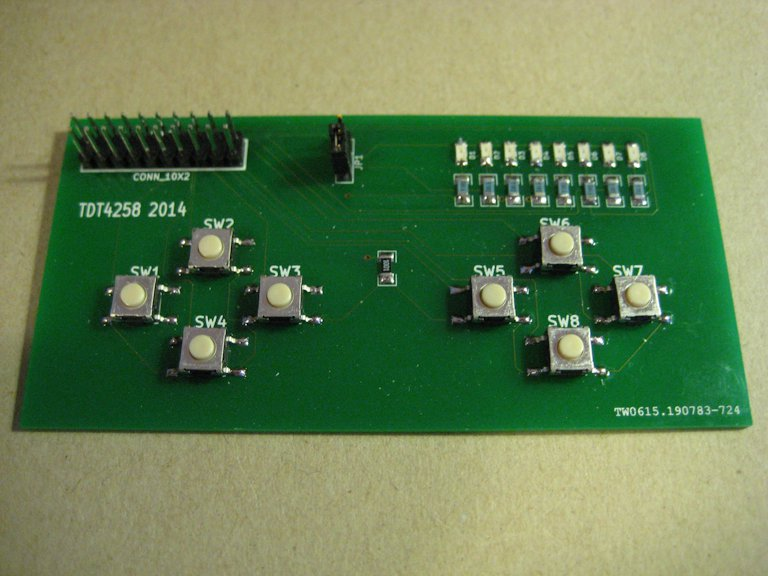
\includegraphics[width=0.5\textwidth]{images/gamepad.jpg}
  \caption{The prototype gamepad}\label{fig:gamepad}
\end{figure}


\section{Energy Management Unit}\label{sec:emu}
The Energy Management Unit (EMU) manages the different low energy modes in the EFM32GG. The EFM32GG has the capability to turn off power to board components at runtime by switching between five distinct energy modes. These modes range from EM0 (run mode) where the CPU and all peripherals are active, to EM4 where almost everything is disabled. The hardware component map in figure \ref{fig:giant-gecko-map} shows what components are active in the different energy modes by showing them with separate colors. A darker color indicates a component that is available in a lower energy mode. In addition to handling the energy modes, the EMU can also be used to turn off the power to unused SRAM blocks.\cite{efm32gg-rm}
% TODO(maybe): Explain how to disable RAM blocks
% TODO(maybe): Write more about the different energy modes


\section{Low Energy Timer}\label{sec:letimer}
The Low Energy Timer (LETIMER) is a 16-bit timer available in energy modes down to EM3. Similar to the TIMER module (section \ref{sec:timer}), it can be used to generate interrupts after specific time intervals, to generate PRS signals for other peripherals, and to generate arbitrary waveforms on its two output pins. The fact that the LETIMER is available in EM3 makes it especially useful for applications where energy consumption is at a minimum. As mentioned in section \ref{sec:cmu}, the LETIMER is driven by the Low Frequency A Clock.

The LETIMER can be started and stopped by setting the START and STOP bits respectively in register LETIMER0\_CMD. It has an internal counter that is decremented each cycle, and that can be read from register LETIMER0\_CNT. The counter value is by default reloaded to \texttt{0xffff} when it underflows, but this can be changed by setting COMP0\_TOP in LETIMER0\_CTRL and writing a new reload value to LETIMER0\_COMP0. 


\section{Peripheral Reflex System}\label{sec:prs}
The Peripheral Reflex System (PRS) is a network connecting the different peripheral modules together, allowing them to communicate directly without involving the CPU. The peripheral modules send each other \emph{reflex signals} routed by the PRS. On receiving such a signal, a peripheral module may perform some specific action depending on the signal received. By relieving the CPU of work, the PRS system can be used to improve energy efficiency. It is also suited for time-critical operations as it involves no variable-time software overhead.


%\section{Low Energy Universal Asynchronous Receiver/Transmitter}\label{subsec:leuart}
%TODO % TODO


\section{Direct Memory Access controller}
Direct Memory Access (DMA) is a technique in which I/O devices use the CPU bus to access the memory directly without involving the CPU. 
% TODO(maybe): Mention benefits of offloading work from the CPU
This is usually achieved by having a DMA controller, a specialized hardware component that can transfer data between memory and I/O devices, without direct interaction from the CPU. The I/O devices will be unaware that the transfer is being done by the DMA controller and not the CPU. An alternative to using a DMA controller for I/O is to do programmed input/output, where the CPU either uses interrupts or busy-wait to continually service an I/O device. DMA usually benefits over this approach as it allows the CPU to perform other work, or to enter low energy modes.
% TODO(maybe): Mention bus clogging and CPU idling. How can the DMA share a bus with the CPU?
It is possible to run the DMA in EM2 by using the LEUART module (see section \ref{subsec:leuart}).

\subsection{Configuration and use}
The DMA controller has 12 independent \emph{channels}. These can be triggered from either peripherals or software to start a DMA cycle. During a cycle, the DMA controller will read a \emph{channel descriptor} from system memory corresponding to that channel(?), and perform one or more DMA transfers as specified by the channel descriptor (and the DMA configuration?).

\subsubsection{Channel Configuration}
Before using a peripheral module together with the controller, a DMA channel must be configured to receive that peripheral's requests. This is done by writing to the channel control registers DMA\_CHx\_CTRL. These registers have two components: SOURCESEL, used to select which peripheral to listen to, and SIGSEL that specifies the signal to listen to of that peripheral.

\subsubsection{DMA Cycles}
A DMA cycle consists of several DMA transfers in which the controller transfers a single byte or word from one memory location to another. The controller might need several cycles in order to completely service a request. The behaviour of the controller during a cycle must be specified in the channel descriptor by setting a cycle type in the cycle\_ctrl bits.

\subsubsection{Channel Descriptors}
Channel descriptors are used to configure the behaviour of the DMA controller during a single DMA cycle. The channel descriptors must be stored in a contiguous area of memory called the \emph{channel control data structure}. The channel controll data structure itself consists of a primary and an alternate data structure, and these are lists of channel descriptors. It is the responsibility of the software to allocate the channel control data structures, and to write the channel descriptors needed. In addition, the base address of the channel control data structure needs to be written to the controller register DMA\_CTRLBASE. When reading the channel control data structure, the controller uses the lower eight bits to address channel descriptors. For this reason, the base address of the data structure must be at an address like 0xXXXXXX00.

A channel descriptor contains the following elements:
\begin{itemize}
	\item src\_data\_end\_ptr, a pointer to the ending address of the source data.
	\item dst\_data\_end\_ptr, a pointer to the ending address of the destination data.
	\item channel\_cfg, provides control information such as cycle type and R\_power.
\end{itemize}
At the start of a DMA cycle, the controller will read the channel\_cfg from memory. After completing the cycle, an updated channel\_cfg will be written back.



\section{Energy Optimization}
This section introduces relevant theory of energy optimization, and lists several energy optimization techniques that are used in modern computing.

\subsection{Static and dynamic power}
When considering the power consumption of an electronic CMOS integrated circuit, it is useful to split the power into two main parts: \emph{dynamic power} and \emph{static power}. 

Dynamic power is the power needed to switch a circuit between two states. It depends on the clock frequency and activity level of a circuit, and is proportional to the square of the circuit voltage. In a clocked circuit it can be expressed as
$$P_{dynamic} = \alpha CV_{DD}^{2}f$$
where $\alpha$ is the activity level, $C$ is the capitance, $V_{DD}$ is the voltage, and $f$ is the clock frequency of the circuit.

Static power is power that dissipates due to leakage in the transistors of a circuit. It is linearly proportional to the circuit voltage, but independent of frequency. Static power can be expressed as
$$P_{static} = I_{leak}V_{DD}$$
where $I_{leak}$ is the current leaking through the transistors.

The total power used by the circuit is the sum of both dynamic and static power,
$$P_{total} = P_{dynamic} + P_{static}\ .$$
\cite{cmos-vlsi-design}


\subsection{EFM32GG Energy Optimization Techniques}
This section gives an overview of several ways to reduce the static and dynamic power consumption in the EFM32GG.

\subsubsection{Clock Gating}
Clock gating is a technique that reduces dynamic power consumption by disconnecting the clock from unused circuits. The EFM32GG uses automatic clock gating, and supports manual clock gating of both core modules and peripherals on an individual basis (see section \ref{sec:cmu}). Some energy can be saved by turning clocks on and off as the individual peripherals are needed.\cite{efm32-energy-optimization} 


\subsubsection{Disabling RAM blocks}
In the EFM32GG there is a static power dissipation in the RAM blocks of approximately 170 nA per 32 KB block. This constitutes a considerable amount when the device is in EM2 or EM3 energy modes. The RAM blocks can be disabled individually, and this is explained in section \ref{sec:emu}.\cite{efm32-energy-optimization}


\subsubsection{Increasing CPU frequency}
By increasing the clock frequency of the CPU it is possible to reduce its overall static power consumption. An increased frequency usually means that the CPU will finish its computations sooner, allowing it to stay in low energy modes for a larger fraction of the time. Increasing the frequency will also cause an increase in dynamic power consumption, but this is cancelled out by the similar reduction in processing time. There are some exceptional cases where the CPU processing speed is limited by wait-states in bus protocols. In such a case, the frequency should be increased within the imposed bounds.\cite{efm32-energy-optimization}


\subsubsection{Optimizing peripheral clocks}
The EFM32GG has several clocks and oscilliators running at different frequencies. By using a slower clock for the peripherals, the associated dynamic power consumption is reduced. It is optimal to selecting the slowest clock that satisfies the application requirements. Clock prescalers in the CMU or the individual peripherals can be used to adjust the frequency further. Clocks and oscilliators are controlled by the Clock Management Unit, described in section \ref{sec:cmu}.\cite{efm32-energy-optimization} 
% Relevant optimization techniques:
%  - Changing prescalers on-the-go to run at the fastest possible speed without introducing wait-states


\subsubsection{Reducing Bias Current of Analog Peripherals}
Most analog peripherals in the EFM32GG use something called a \emph{bias current}. It is possible to reduce this bias current to reduce power consumption, but this will affect the analog performance.\cite{efm32-energy-optimization}
% TODO(maybe): Expand this section by explaining what a bias current is


\subsubsection{Cache Optimization}
Several optimizations can be made by utilizing the caches of the EFM32GG. When a memory read or instruction fetch is satisfied from the cache, the processor avoids possible wait-states and memory reads and energy is saved. To optimize use of the 512 byte instruction cache of the EFM32GG, loops with a large number of instructions should be avoided. It is possible to measure cache misses and cache hits by reading performance counter registers.\cite{efm32-energy-optimization}
% TODO(optional): Write more about data caches in the EFM32GG. Should possibly be in a different section.


\subsubsection{Compiler optimizations}
As a rule of thumb, using a higher compiler optimization-level will result in more energy-efficient code.
% Relevant optimization techniques:
%  - optimizing for smaller program size vs speed


%--------------------------------------------------------------------
% Other optimization techniques that might be put into this section: 
% (from the Energy Optization Application Note)
%
%  - Use interrupts instead of busy wait
%  - Use wait-for-event instead of interrupts
%  - Use peripheral reflex system
%  - Saving power with DMA
%--------------------------------------------------------------------


\section{Sounds Generation}\label{sec:sound-generation}
When interpreting a sound as a signal, we speak about properties of the sound such as frequency, period, and amplitude. Here frequency and period (the inverse frequency) describes the pitch of a sound, while amplitude describes the loudness. In a typical speaker, a voltage signal is converted directly into sound waves. Here the voltage signal is an accurate model of the sound wave and has the same frequency and amplitude. The range of sounds that can be perceived by a human being is from 20Hz to 20KHz.\cite{compendium}
% TODO: Write about how different tones can be generated

\subsection{Simple music theory}
In the western world the chromatic scale is the standard way to describe music. The chromatic scale is a set of 12 ordered frequences such that the twelwth note has twice the frequency of the first, and that the spacing between the notes is equal on a logarithmic scale. The common ground note in western music is the $A_{4}$ with the frequency of 440hz. The number refers to the octave, such that $A_{5}$ at one octave higher will have twice the frequency of $A_{4}$, 880hz. The note is the letter, and can be sharpened with a \#. The 12 notes on a chromatic scale will be referred to as A, A\#/H, B, C, C\#, D, D\#, E, F, F\#, G, G\#. There is no differenence between a note with a \# and one without, they all have the same relation to their predecessor. \\
The frequency of a note is given by the following equation: $$f = A_{4}*2^{D/12}$$
Here we have used $A_4$ as the ground note, and D is the difference. For instance a third octave C sharp $C\#_3$ is 7 tones lower than $A_4$, so its frequency f will be $$f_{C\#_{3}} = f_{A_{4}}*2^{-7/12}$$
